\documentclass[14pt, oneside]{altsu-report}

\worktype{Отчёт по практике на тему:}
\title{Создание игры на Godot}
\author{Н.\,А.~Павленко}
\groupnumber{5.205-2}
\GradebookNumber{1337}
\supervisor{И.\,А.~Шмаков}
\supervisordegree{ст. пр. к. ВТиЭ}
\ministry{Министерство науки и высшего образования}
\country{Российской Федерации}
\fulluniversityname{ФГБОУ ВО Алтайский государственный университет}
\institute{Институт цифровых технологий, электроники и физики}
\department{Кафедра вычислительной техники и электроники}
\departmentchief{В.\,В.~Пашнев}
\departmentchiefdegree{к.ф.-м.н., доцент}
\shortdepartment{ВТиЭ}
\abstractRU{Большой текст на русском! Пока счётчик работает не правильно! Поправьте количество рисунков и таблиц в cls-файле.}
\abstractEN{Большой текст на английском!}
\keysRU{компьютерное моделирование, cистема управления версиями}
\keysEN{computer simulation, distributed version control}

\date{\the\year}

% Подключение файлов с библиотекой.
\addbibresource{graduate-students.bib}

% Пакет для отладки отступов.
%\usepackage{showframe}

\begin{document}
\maketitle

\setcounter{page}{2}
\makeabstract
\tableofcontents

\chapter*{Введение}
\phantomsection\addcontentsline{toc}{chapter}{ВВЕДЕНИЕ}

\textbf{Актуальность}

\textbf{Цель}

\textbf{Задачи:}
\begin{enumerate}
\item Текст много текста.
\item Текст много текста.
\item Текст много текста.
\end{enumerate}

% Подключение первой главы (теория):
\chapter{\label{ch:ch01}ГЛАВА 1. Обзор Godot} % Нужно сделать главу в содержании заглавными буквами

\section{\label{sec:ch01/sec01}Раздел 1. Возможности Godot}

\subsection{\label{subsec:ch01/sec01/sub01}Описание движка}

Godot - это универсальный и простой в освоении игровой движок, который позволяет создавать как 2D, так и 3D игры. Он обладает широким спектром возможностей, делающих его привлекательным выбором как для начинающих, так и для опытных разработчиков.

\subsection{\label{subsec:ch01/sec01/sub02}2D и 3D возможности Godot}

\textbf{2D:}

\begin{itemize}
    \item Создание 2D персонажей, окружения и интерфейсов.
    \item Плавная анимация с использованием спрайтов, скелетной анимации и tween-инструментов.
    \item Физика 2D с реалистичными столкновениями и взаимодействиями.
    \item Tilemaps для создания уровней с повторяющимися элементами.
    \item Камеры с эффектами параллакса, приближения и тряски.
    \item Частицы для создания визуальных эффектов, таких как взрывы, дождь и огонь.
\end{itemize}

\textbf{3D:}

\begin{itemize}
    \item 3D моделирование и импорт из популярных форматов (OBJ, FBX и т.д.).
    \item PBR-шейдеры для реалистичного освещения и материалов.
    \item Физика 3D с Bullet Physics Engine.
    \item Анимация персонажей с использованием скелетной анимации.
    \item Редактор для создания 3D ландшафтов.
    \item Эффекты пост-обработки для лучшего визуального качества игры.
\end{itemize}


\subsection{\label{subsec:ch01/sec01/sub02}Система, основанная на "нодах"}

Godot использует уникальную node-based систему для организации игровых объектов и их взаимодействия. Это позволяет разработчикам легко создавать сложные сцены и управлять объектами через иерархию узлов. У каждого "нода" есть свои параметры и "дети" которые наследуют некоторые характеристики "родителя", что позволяет создавать различные взаимодействия между объектами чуть легче, чем в других движках.

\section{\label{sec:ch01/sec02}Раздел 2: много уровневые списки}

\subsection{\label{subsec:ch01/sec02/sub01}Подраздел 1: пример нумерованного списка}

Пример вложенного нумерованного списка:
\begin{enumerate}
\item Первый элемент:
\begin{enumerate}
\item Первый элемент первого элемента;
\item Второй элемент первого элемента;
\end{enumerate}
\item Второй элемент:
\begin{enumerate}
\item Первый элемент второго элемента;
\item Второй элемент второго элемента.
\end{enumerate}
\end{enumerate}

\subsection{\label{subsec:ch01/sec02/sub02}Подраздел 2: пример маркерованного списка}

Пример вложенного маркерованного списка:
\begin{itemize}
\item первый элемент:
\begin{itemize}
\item первый элемент первого элемента;
\item второй элемент первого элемента;
\end{itemize}
\item Второй элемент:
\begin{itemize}
\item первый элемент второго элемента;
\item второй элемент второго элемента.
\end{itemize}
\end{itemize}

Пример ссылки на рисунок в документе~\ref{fig:example01}.
\begin{figure}[h]
    \centering
    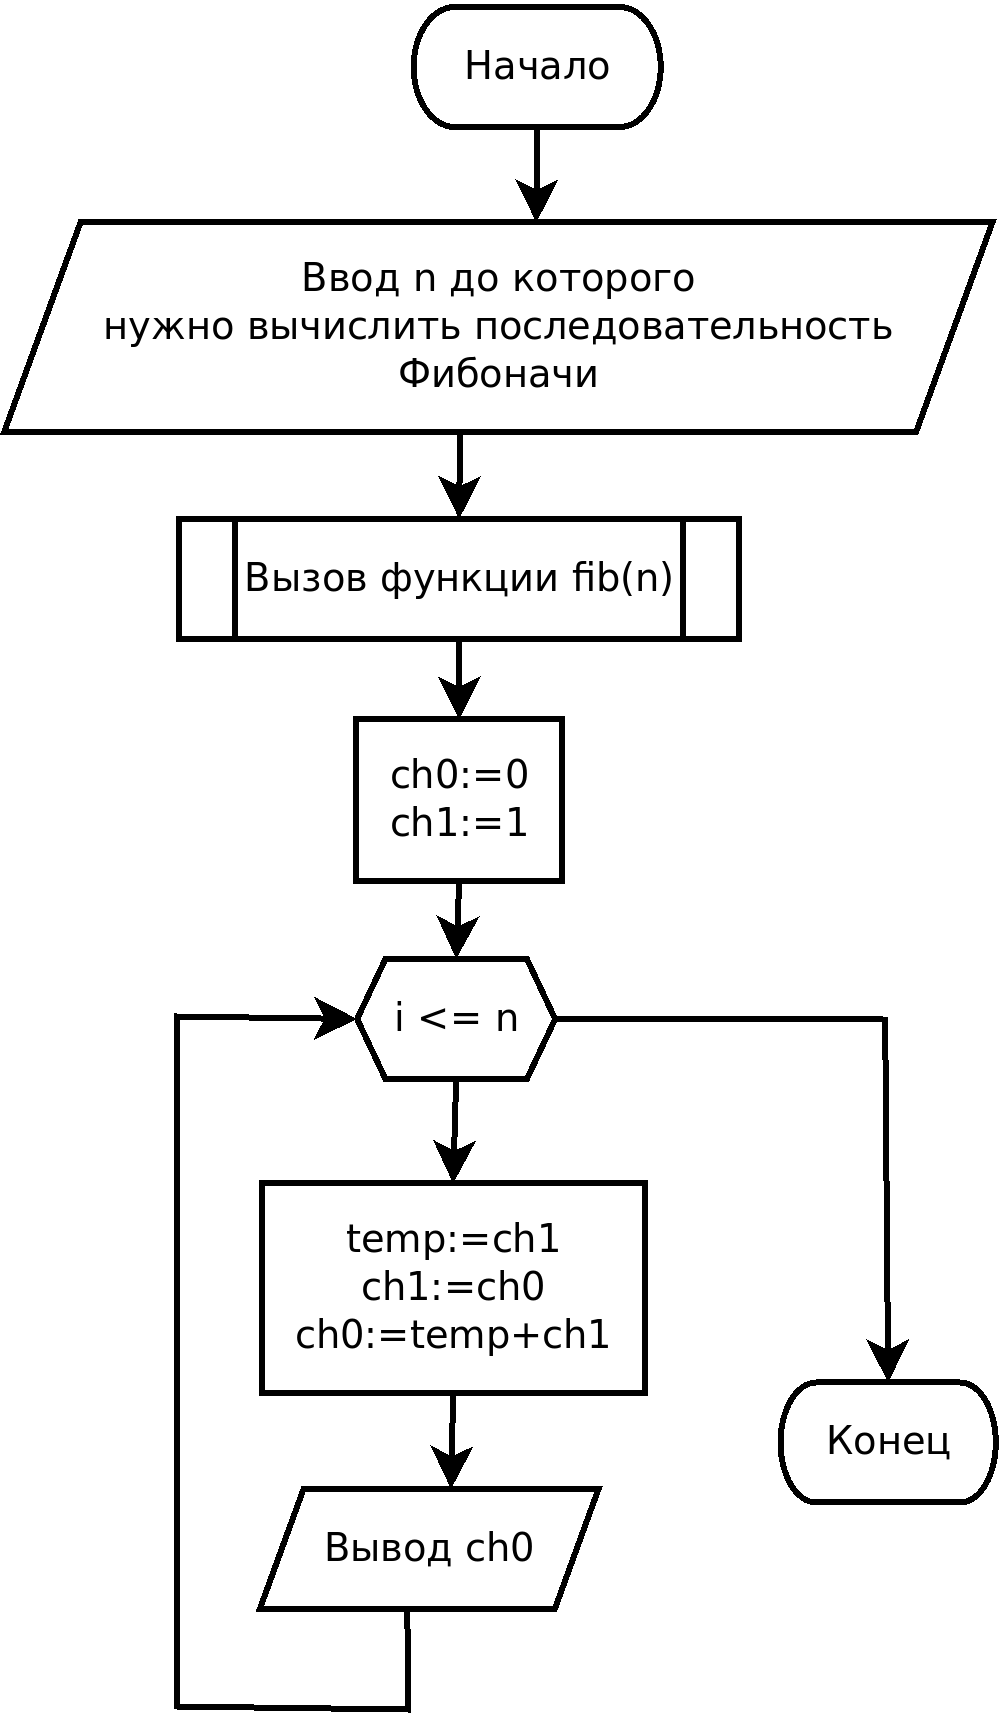
\includegraphics[width=0.5\textwidth]{./images/fibonacci.png}
    \caption{\centering\label{fig:example01}Пример рисунка в формате PNG.}
\end{figure}

Пример ссылки на рисунок в документе~\ref{fig:example02}.
\begin{figure}[h]
    \centering
    \includesvg[width=0.5\textwidth]{./images/fibonacci.svg}
    \caption{\centering\label{fig:example02}Пример рисунка в формате SVG.}
\end{figure}

Пример ссылки на таблицу в документе~\ref{tab:example01}.
\begin{table}[H]
\caption{\centering\label{tab:example01}Системные требования}
\begin{tabular}{|p{3 cm}|p{3 cm}|p{3 cm}|p{5 cm}|}
\hline
Минимальные требования & 1 & 2 & 3 \\ \hline
Версия операционной системы & 1 & 2 & 3 \\ \hline
Процессор & 1 & 2 & 3 \\ \hline
Графический API & 1 & 2 & 3 \\ \hline
\end{tabular}
\end{table}

Пример ссылки на таблицу в документе~\ref{tab:example02}.
\begin{table}[H]
\caption{\centering\label{tab:example02}Системные требования}
\begin{tabular}{|p{3 cm}|p{3 cm}|p{3 cm}|p{5 cm}|}
\hline
Минимальные требования & 1 & 2 & 3 \\ \hline
Версия операционной системы & 1 & 2 & 3 \\ \hline
Процессор & 1 & 2 & 3 \\ \hline
Графический API & 1 & 2 & 3 \\ \hline
\end{tabular}
\end{table}

Пример использования minted для оформления кода и ссылка на этот код~\ref{code:fibonacci}.
\begin{code}
\captionof{listing}{\centering\label{code:fibonacci}Пример программы вычисления n-ой последовательности Фибоначчи}
\vspace{-\baselineskip}\inputminted{python}{src/fibonacci.py}
\end{code}

Пример использования minted для оформления кода и ссылка на этот код~\ref{code:example02}.
\begin{code}
\captionof{listing}{\centering\label{code:example02}Сложение двух массивов параллельно десятью потоками (пример из https://ru.wikipedia.org/wiki/OpenMP)}
\vspace{-\baselineskip}\begin{minted}{C}
#include <stdio.h>
#include <omp.h>
#define N 100

int main(int argc, char *argv[]) {
  double a[N], b[N], c[N];
  int i;
  omp_set_dynamic(0); // запретить библиотеке openmp менять число потоков во время исполнения
  omp_set_num_threads(10); // установить число потоков в 10
  // инициализируем массивы
  for (i = 0; i < N; i++) {
      a[i] = i * 1.0;
      b[i] = i * 2.0;
  }
  // вычисляем сумму массивов
#pragma omp parallel for shared(a, b, c) private(i)
   for (i = 0; i < N; i++)
     c[i] = a[i] + b[i];

  printf ("%f\n", c[10]);
  return 0;
}
\end{minted}
\end{code}

% Подключение второй главы (практическая часть):
\chapter{\label{ch:ch02}ГЛАВА 2. Разработка игры}

\section{\label{sec:ch02/sec01}Раздел 1. Проектирование игрового процесса и механик}

\subsection{\label{subsec:ch02/sec01/sub01}Подраздел 1. Анализ классической Asteroids и определение основных игровых механик}

Анализ основной игры "Asteroids". Ключевые механики:
\begin{itemize}
    \item Управление игровым кораблем в открытом космосе с возможностью перемещения во всех направлениях.
    \item Разрушение астероидов при помощи снарядов, ведущее к их разделению на более мелкие части.
    \item Опасность столкновения с астероидами и другими объектами на игровом поле, что приводит к потере жизней игрока или поражению.
    \item Система отсчета очков, мотивирующая игрока к достижению новых рекордов и улучшению своих результатов.
\end{itemize}

Новые механики:
\begin{itemize}
    \item Выбор сложности в меню настроек, от сложности зависит количество осколков на которые разделяется астероид, их размер, и количество очков, которое дается за их уничтожение.
    \item Онлайн таблица лидеров в реальном времени, после конца игры можно записать себя в таблицу лидеров под любым именем.
    \item Система бонусов и усилений, которые помогают игроку в сражении с астероидами и увеличивают его шансы на выживание.
    \item Различные визуальные и звуковые эффекты для лучшего игрового опыта.
\end{itemize}


\subsection{\label{subsec:ch02/sec01/sub02}Подраздел 2. Определение целей игры, основных действий игрока и правил игрового процесса}

Основные цели, задачи и правила игры:
\begin{itemize}
    \item Цель игры: выжить как можно дольше, уничтожая астероиды и избегая столкновений с ними и другими объектами.
    \item Основные действия игрока: управление кораблем, стрельба по астероидам, уклонение от опасностей и сбор бонусов.
    \item Правила игрового процесса: игрок начинает игру в центре экрана и пытается набрать максимальное количество очков, избегая столкновений и уничтожая астероиды.
\end{itemize}

\subsection{\label{subsec:ch02/sec01/sub03}Подраздел 3. Создание концепции игры, включая уровни сложности, прогрессию и целевые достижения}

Общая концепция игры "Asteroids", включающая:
\begin{itemize}
    \item Уровни сложности: планируется создание нескольких уровней, каждый из которых будет характеризоваться увеличивающимся количеством и скоростью астероидов, а также другими усложнениями игрового процесса.
    \item Прогрессия: игра будет предусматривать систему постепенного увеличения сложности, чтобы поддерживать интерес игрока и давать ему возможность постоянно улучшать свои навыки.
    \item Целевые достижения: будут определены определенные цели и достижения, например, достижение определенного количества очков, продержаться определенное время или уничтожить определенное количество астероидов.
\end{itemize}

\section{\label{sec:ch02/sec01}Раздел 2. Проектирование и реализация игрового корабля}

- Разработка внешнего вида игрового корабля с учетом эстетических и функциональных требований
- Создание анимаций для игрового корабля, включая анимацию движения, выстрелов и уничтожения
- Реализация управления игровым кораблем с использованием клавиатуры, мыши или других устройств ввода
- Программирование взаимодействия игрового корабля с окружающим миром, такое как столкновения с астероидами и другими игровыми объектами

\subsection{\label{subsec:ch02/sec01/sub01}Подраздел 1. Разработка внешнего вида игрового корабля}

Корабль представлен простым белым треугольником, сзади которого при движении выпускаются эффекты огня (работы двигателя), стреляет корабль из своего "носа" желтыми круглыми пулями.

\begin{figure}
    \centering
    
\includegraphics[width=0.5\linewidth]{images/spaceship.png}
    \caption{Космический корабль}
    \label{fig:enter-label}
\end{figure}

\subsection{\label{subsec:ch02/sec01/sub02}Подраздел 2. Реализация управления игровым кораблем}


Реализация управления игровым кораблем в скрипте player.gd~\ref{code:example01}.
\begin{code}
\captionof{listing}{\centering\label{code:example01}Код для движения корабля}
\vspace{-\baselineskip}\begin{minted}{C}
func move(delta):
    # Задаем направление поворота персонажа
    rotation_direction = Input.get_axis("ui_left", "ui_right")
    # Проверяем нажата ли клавиша для движения вперед
    is_moving = Input.is_action_pressed("forward")

    # Поворот персонажа при нажатии клавиш
    if rotation_direction > 0:
        rotation += rotation_speed * delta
    elif rotation_direction < 0:
        rotation -= rotation_speed * delta

    # Если клавиша вперед нажата двигаемся вперед относительно поворота персонажа
    # И замедляемся, при отжатии клавиши
    if is_moving:
        velocity += Vector2(0, 1).rotated(rotation) * speed
    else:
        velocity = velocity.move_toward(Vector2.ZERO, deceleration)
    velocity = velocity.clamp(-max_speed_vector, max_speed_vector)
\end{minted}
\end{code}

Функция "move" находится в основной функции \_physics\_process(delta), которая обновляется каждый кадр, где delta - разность во времени между двумя кадрами.

\subsection{\label{subsec:ch02/sec01/sub03}Подраздел 3. Программирование взаимодействия игрового корабля с окружающим миром}

При столкновении с астероидом конец игры и переход в следующую сцену~\ref{code:example02}.
\begin{code}
\captionof{listing}{\centering\label{code:example02}Код для конца игры}
\vspace{-\baselineskip}\begin{minted}{C}
func _on_collision_player_body_entered(body):
    if body is Enemy:
        die()


func die():
    get_tree().change_scene_to_file("res://Scenes/end_screen.tscn")
\end{minted}
\end{code}


Перемещение персонажа при достижении края экрана~\ref{code:example03}.
\begin{code}
\captionof{listing}{\centering\label{code:example03}Код для перемещения персонажа при достижении края экрана}
\vspace{-\baselineskip}\begin{minted}{C}
func out_of_bounds():
    position = position.posmodv(screen_size)
\end{minted}
\end{code}


Реализация стрельбы при нажатии определенной кнопки и реализация улучшения "тройной выстрел"~\ref{code:example03}.
\begin{code}
\captionof{listing}{\centering\label{code:example03}Код для стрельбы}
\vspace{-\baselineskip}\begin{minted}{C}
func shoot():
    bullet_timer -= 1

    if !can_shoot and bullet_timer <= 0:
        can_shoot = true
        bullet_timer = 20

    if can_shoot and Input.is_action_just_pressed("shoot"):
        $AudioStreamPlayer.pitch_scale = randf_range(0.8, 1.6)
        $AudioStreamPlayer.playing = true

        can_shoot = false
        var bullet = BULLET_PATH.instantiate()
        if Globals.triple_shot:
            var bullet2 = bullet.duplicate()
            bullet2.global_position = $Marker2D.global_position + Vector2(10, 10)
            bullet2.velocity = Vector2(0, 1).rotated(rotation) * bullet_speed
            bullet2.scale = Vector2(0.1, 0.1)
            var bullet3 = bullet.duplicate()
            bullet3.global_position = $Marker2D.global_position + Vector2(-10, -10)
            bullet3.velocity = Vector2(0, 1).rotated(rotation) * bullet_speed
            bullet3.scale = Vector2(0.1, 0.1)
            get_parent().add_child(bullet2)
            get_parent().add_child(bullet3)
        bullet.scale = Vector2(0.1, 0.1)

        get_parent().add_child(bullet)
        bullet.position = $Marker2D.global_position
        bullet.velocity = Vector2(0, 1).rotated(rotation) * bullet_speed
\end{minted}
\end{code}

\section{\label{sec:ch02/sec03}Раздел 3. Добавление звуковых эффектов и музыки}

\begin{itemize}
    \item Подбор и добавление звуковых эффектов для различных игровых событий, таких как выстрелы, взрывы и столкновения с помощью сайта \cite{https://sfxr.me/}
    \item Интеграция фоновой музыки для создания атмосферы игры и поддержания интереса игрока. Фоновая музыка (с разрешения автора) \cite{https://www.youtube.com/watch?v=-35AC-FPoAA}
    \item Настройка звуковых уведомлений и звуковых сигналов для обратной связи с пользователем, также с помощью сайта \cite{https://sfxr.me/}
\end{itemize}
 
% Подключение третий главы (практическая часть с тестированием:
\chapter{\label{ch:ch03}ГЛАВА 3. Тестирование игры и исправление ошибок}



\chapter*{Заключение}
\phantomsection\addcontentsline{toc}{chapter}{ЗАКЛЮЧЕНИЕ}

\begin{enumerate}
\item Пример ссылки на электронный источник~\cite{wikiRUBitbucket,wikiRUIdSoftware,wikiRUGitHub}.
\item Пример ссылки на книгу одного автора~\cite{book1author}.
\item Пример ссылки на книгу 5-ти и более авторов~\cite{book5author}.
\end{enumerate}

\newpage
\phantomsection\addcontentsline{toc}{chapter}{СПИСОК ИСПОЛЬЗОВАННОЙ ЛИТЕРАТУРЫ}
\printbibliography[title={Список использованной литературы}]

\appendix
\newpage
\chapter*{\raggedleft\label{appendix1}Приложение}
\phantomsection\addcontentsline{toc}{chapter}{ПРИЛОЖЕНИЕ}
%\section*{\centering\label{code:appendix}Текст программы}

\begin{center}
\label{code:appendix}Текст программы
\end{center}

\begin{code}
\captionof*{listing}{\centering\label{code:pi-example}Пример программы вычисления числа $\pi$ на языке \textit{C} с использованием \textit{MPI} (пример из https://ru.wikipedia
.org/wiki/Message\_Passing\_Interface)}
\vspace{-1cm}\inputminted{C}{src/pi-mpi.c}
\end{code}

\end{document}

